\chapter{Similarity and Scaling} %(notes page 67-71)
\label{sec:SimilarityAndScaling}
\index{similarity}
\index{scaling}

Locomotives come in a variety of sizes. It is often possible to draw valuable conclusions about the dynamics of locomotion if the motion of different locomotives is compared. The comparison of different locomotives often requires the consideration of the different scales between the locomotives. An examination of scaling between locomotives can provide information about the relative sizes of limbs between animals, the period of a gait, and more importantly the metabolic cost of locomotion \cite{mcmahon84}. Additionally, scaling can be used to predict the speed at which similar animals transition between gaits (e.g. walking to running). 

\begin{comment}As one example, in the simplest walker model of locomotion (section \ref{sec:SimplestWalker}) the slope of the incline is related to the stance leg angle $\theta_{1}^{*}$ that is required for stable motions \cite{garcia97}. GARCIA 97, SIMPLEST WALKER PAPER, TALKS ABOUT SCALING OF STANCE LEG ANGLE WITH SLOPE, BUT THIS IS NOT THE SAME SCALING
[chris: the above paragraph should be edited to give a better sense of why we're doing this]
\end{comment}

Two systems are similar if they can be made identical by simple rescaling. This means that after rescaling, the two systems have the same shape, the same physical properties, the same governing equations, and the same solutions. One type of similarity is geometric similarity, in which two systems have exactly the same shape but have a different size. A simple case of geometric similarity is that of similar triangles.

% FIGURE
\begin{figure}[h]		% h="here" t="top" b="bottom" p="separate page"
\begin{centering}
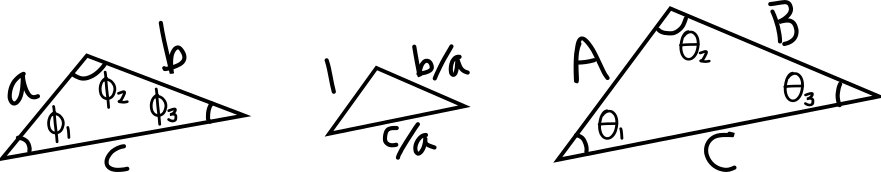
\includegraphics[width=0.7\textwidth]{Figures/GeometricScaling}\par
\end{centering}
\caption[Diagram: Geometric Scaling of Triangles]{Geometric scaling of triangles. The left triangle and right triangle are similar to each other if $a/A = b/B = c/C$, $\phi_{i} = \theta_{i}$. The middle triangle is a generalized nondimensional triangle representing the two similar ones. The ideas of geometric scaling can be useful in locomotion.}
\label{fig:GeometricScaling}
\end{figure}
%

The leftmost and rightmost triangles in figure \ref{fig:GeometricScaling} are similar if $a/A = b/B = c/C$, $\phi_{1} = \theta_{1}, \phi_{2} = \theta_{2}, and \phi_{3} = \theta_{3}$. Additionally, if the area of the leftmost triangle is $\beta a^2$, then the area of the rightmost triangle is $\beta A^2$, where $\beta$ is a parameter given by the shape of the similar triangles.

The process of scaling often entails developing nondimensionalized models and equations. This means that key parameters of a system are scaled (divided) by logical constants that have the same units as the key parameter. For the geometric case of triangles, the nondimensionalized triangle is given by the middle triangle in figure \ref{fig:GeometricScaling} (angles are already or dimensionless). The leftmost and rightmost triangles can then be described by the nondimensionalized, or generalized, triangle and a single scaling factor: $a$ for the left triangle, $A$ for the right triangle. Suppose a triangle is used to model some interesting physics. If the model is based on a nondimensionalized triangle, then the model is correct for the infinite set of triangles that are similar to that generalized triangle. 

\subsection{The Generalized Pendulum}

The ideas of scaling are applied to the prototypical dynamics system: the point mass pendulum. The pendulum is described by figure \ref{fig:Pendulum}.

% FIGURE
\begin{figure}[h]		% h="here" t="top" b="bottom" p="separate page"
\begin{centering}
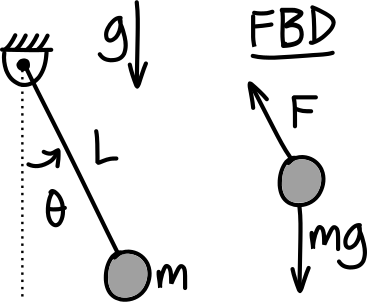
\includegraphics[width=0.25\textwidth]{Figures/Pendulum}\par
\end{centering}
\caption[Diagram: Point Mass Pendulum]{Point mass pendulum. A mass $m$ in Earth's gravity field is attached to a pin by a massless rigid link of length $L$. The rotation of the mass is $\theta$ relative to the vertical. This simple model can be generalized, and equations of motion can be formed that describe any similar pendulum.}
\label{fig:Pendulum}
\end{figure}
%

We desire to generalize the model of the pendulum, so that a single model can be applied to any \textit{similar} pendulum. To generalize this model, we list the variables that describe the model and parameters, the reference quantities for each of the variables, and the nondimensional form of those variables. The nondimensional form of a variable is the actual variable normalized by its reference quantity. A model of a pendulum requires the variables of mass $m$,  length $L$, and the parameter of acceleration due to gravity $g$. The nondimensional variables of the system are $m^{*}$ for mass, $L^{*}$ for length, and $t^{*}$ for time. These are nondimensionalized using the reference quantities, with actual units, $m_{0}, L_{0}$ and $t_{0}$. A characteristic reference time is chosen for the system,

\begin{equation}
t_{0} = \sqrt{\frac{g}{L}}
\label{eq:SimilarCharacteristicTime}
\end{equation}

This form for the reference time is chosen because terms in the expression will cause cancellations with terms that typically arise in the equations of motion. In general, an expression for the reference time arises naturally from the description of the model. The dimensionless variables are

\begin{align}
m^{*} = m/m_{0} \\
L^{*} = L/L_{0} \\
t^{*} = t/t_{0} = t/\sqrt{L/g}
\end{align}

Now, the system's variables have been nondimensionalized. There are two unknowns in the pendulum problem: the rotation of the pendulum arm $\theta(t)$ and the tension in the arm $F(t)$. The first unknown, $\theta(t)$, is determined by a linear momentum balance perpendicular to the arm of the pendulum. Since $\theta(t)$ is dimensionless, there is no need to define a $\theta^{*}$.  The typical equation of motion for a pendulum is

\begin{equation}
\frac{d^{2}}{dt^{2}}\theta + \frac{g}{L} \sin{\theta} = 0 
\end{equation}

This is provided here without derivation. To nondimensionalize this equation, $t$ is replaced with $t^{*}$ from equation \ref{eq:SimilarCharacteristicTime}. 

\begin{equation}
\frac{d^{2}}{d\left(\sqrt{\frac{L}{g}}t^{*}\right)^{2}}\theta + \frac{g}{L} \sin{\theta} = 0  
\end{equation}

The constant term is moved outside of the differential, and cancels with the coefficient of $\sin{\theta}$. 

\begin{equation}
\frac{d^{2}}{dt^{*^{2}}}\theta + \sin{\theta} = 0
\label{eq:SimilarPendulumLMB1}
\end{equation}

This differential equation then describes the motion of all pendulums that are similar to the one in figure \ref{fig:Pendulum}. 

Equation \ref{eq:SimilarPendulumLMB1} provides the motion of any similar pendulum, but does not describe the force that results from this motion. The force of interest here is the tension $F(t)$ in the arm of the pendulum. The tension is determined from linear momentum balance along the arm of the pendulum. Under the small angle approximation $\cos{\theta} = 1$ the free body diagram in figure \ref{fig:Pendulum} provides 

\begin{equation}
F -mg = mL \dot{\theta}^{2}
\label{eq:SimilarForce}
\end{equation} 

Equation \ref{eq:SimilarForce} is generalized

\begin{align}
F &= mg + \left(\frac{d}{dt}\theta\right)^2 mL \notag \\
F &= mg + \left(\frac{d\theta}{d\left(t^{*}\sqrt{L/g}\right)}\right)^2 mL \notag \\
\frac{F}{mg} &= 1 + \left(\frac{d\theta}{dt^{*}}\right)^{2}
\label{eq:SimilarPendulumLMB2}
\end{align}

Each term in equation \ref{eq:SimilarPendulumLMB2} is dimensionless, and we can define a nondimensional tension $F^{*} = F/mg$. The combination of equation \ref{eq:SimilarPendulumLMB1} and equation \ref{eq:SimilarPendulumLMB2} completely describe the dynamics of a generalized pendulum. Of course, this does not mean that \textit{all} pendulums have the same motion in time, or the same arm tension in time. For small oscillations, the period $T$ of oscillation is described by the constant $T^{2}g/L = 4\pi^{2}$. However, a single scaled equation can describe all such pendula. After obtaining a solution, the dimensional form can be found by ``unscaling". For example, $F = mgF^{*}$.

\subsection{Scaling in Locomotion}

Using the same general methodology, the different motion of two similar locomotives can be determined if the two locomotives are scaled properly and a set of dimensionless equations of motion are developed.  

% FIGURE
\begin{figure}[h]		% h="here" t="top" b="bottom" p="separate page"
\begin{centering}
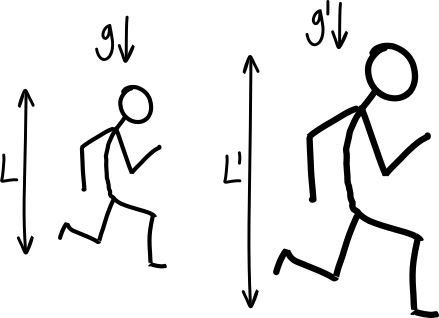
\includegraphics[width=0.4\textwidth]{Figures/ScaledPerson}\par
\end{centering}
\caption[Diagram: Geometric Scaling of a Human]{Geometric scaling of a human. A natural reference length for the scaling of humans is the height $L$ of the human.}
\label{fig:ScaledPerson}
\end{figure}
%

To arrive at solutions for the dynamics, the variables of the system must be nondimensionalized. In general, the following basic reference quantities can be used to develop dimensionless variables.

\begin{itemize}
\item \textbf{Length:} scale by a characteristic length $L_{0}$, e.g. any body part. This is geometric scaling, as in figure \ref{fig:ScaledPerson}.
\item \textbf{Mass:} scale by a characteristic mass $M_{0} \propto \rho L_{0}^{3}$, e.g. total mass.
\item \textbf{Time:} scale by characteristic time $t_{0} = \sqrt{L_{0}/g}$.
\item \textbf{Force:} scale by $M_{0}g$.
\item \textbf{Moments:} scale by $M_{0} g L_{0}$
\end{itemize}

Reference quantities for other important quantities come naturally from those above. If the two locomotives being compared are largely composed of the same material (same density $\rho$), then the mass can be alternatively scaled by $L^{3}$ since $\rho$ is constant. In this case the force can be scaled by $\rho L^{3} g$. Logically, stresses are then scaled as 

\begin{align}
\frac{\mbox{Force}}{\mbox{Area}} &\propto \frac{\rho g L^3}{L^2} \notag \\
\sigma & L
\end{align}

The quantities $\rho$ and $g$ drop out of the proportion because they are constant. A practical example of constant-density geometric scaling is the similarity between mice and elephants (figure \ref{fig:ElephantMouse}). 

% FIGURE
\begin{figure}[h]		% h="here" t="top" b="bottom" p="separate page"
\begin{centering}
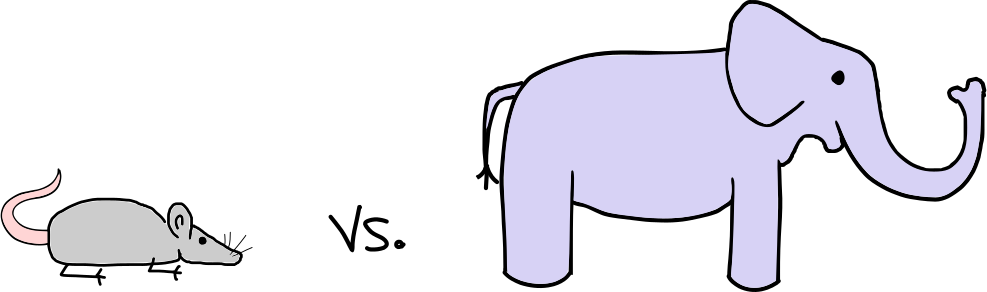
\includegraphics[width=0.9\textwidth]{Figures/ElephantMouse}\par
\end{centering}
\caption[Diagram: Geometric Scaling between Mice and Elephants]{Geometric scaling between mice and elephants. Although apparently unlikely, the similarity of the motion of mice and elephants is revealed through scaling. The two animals are composed of mostly the same material, which simplifies the scaling. However, muscle strength does not scale between the two animals.}
\label{fig:ElephantMouse}
\end{figure}
%
Mice and elephants are close to geometrically similar, and so similar motions between the two animals are possible if the animals are scaled correctly. This means that attributes of locomotion, such as step frequency, are functions of the scaling, e.g. $f(L)$. Additionally, mice and elephants have approximately the same density. As a result, stress (muscle stress) scales as only $\sigma \propto L$. An important feature between mice and elephants that does \textit{not} scale between the two animals (by length, by mass, or otherwise) is muscle strength. The maximum stress that muscles can endure before failing is approximately constant across animals, but the stress induced by a load scales with $L$. For such reasons, an elephant cannot climb a tree as a mouse may.

\begin{comment}
As a result, it is easier to focus on energy considerations. [chris: there should be more here. page 247 of McMahon discusses 3 implications of the fact that maximum stress that muscles can endure is const across scales. however, mcmahon uses a different dimensionless forcein general a lot more research reading needs to go into this stuff. also, like worked examples.].
\end{comment}

A particularly interesting use of scaling is the prediction of \textit{gait transitions}\index{gait transition}. A gait transition, such as that between walking and running, is described by the speed $v_{t}$ at which a locomitve naturally changes its gait. The dimensionless speed of a locomotive is 

\begin{equation}
v^{*} = \frac{v}{\sqrt{gL}}
\end{equation}

This is called the Froude number of locomotion\index{Froude number}. The Froude number appears often in fluid dynamics for scaling purposes, but is relevant here as well. While in general, different animals transition between gaits at different transition speeds $v_{t}$, it has been shown that all animals transition between a walking gait to a running gait at about $v_{t}^{*} = 1$.

So far, we have focused on geometric similarity. While various aspects of locomotion \emph{do} scale with characteristics quantities like $L$, experiments have shown that they do not scale as would be expected by simle geometric scaling. For example, one study shows that stride frequency is proportional to $L^{-.5}$, whereas geometric scaling asserts an $L^{-1}$ relation.

Other types of similarity exist, such as \emph{elastic similarity}. Similarity rules can be developed for different elastic loading scenarios, such as buckling of the leg at the knee joint. Elastic buckling similarity purports that for two similar animals to have the same resistance to the buckling, the limbs' diameter $d$ and length $l$ are related by

\begin{equation}
d \propto l^{3/2}
\end{equation} 

Note that this breaks geometric similarity, which requires $d \propto l$. Thus, it is not always possible for two systems to be similar by multiple standards.

For a more thorough examination of scaling, refer to McMahon \cite{mcmahon84}. McMahon discusses experiments that have been conducted relevant to locomotion scaling, with particular regard to biological function such as blood velocity and life span.







